\begin{figure}[htp]
\centering
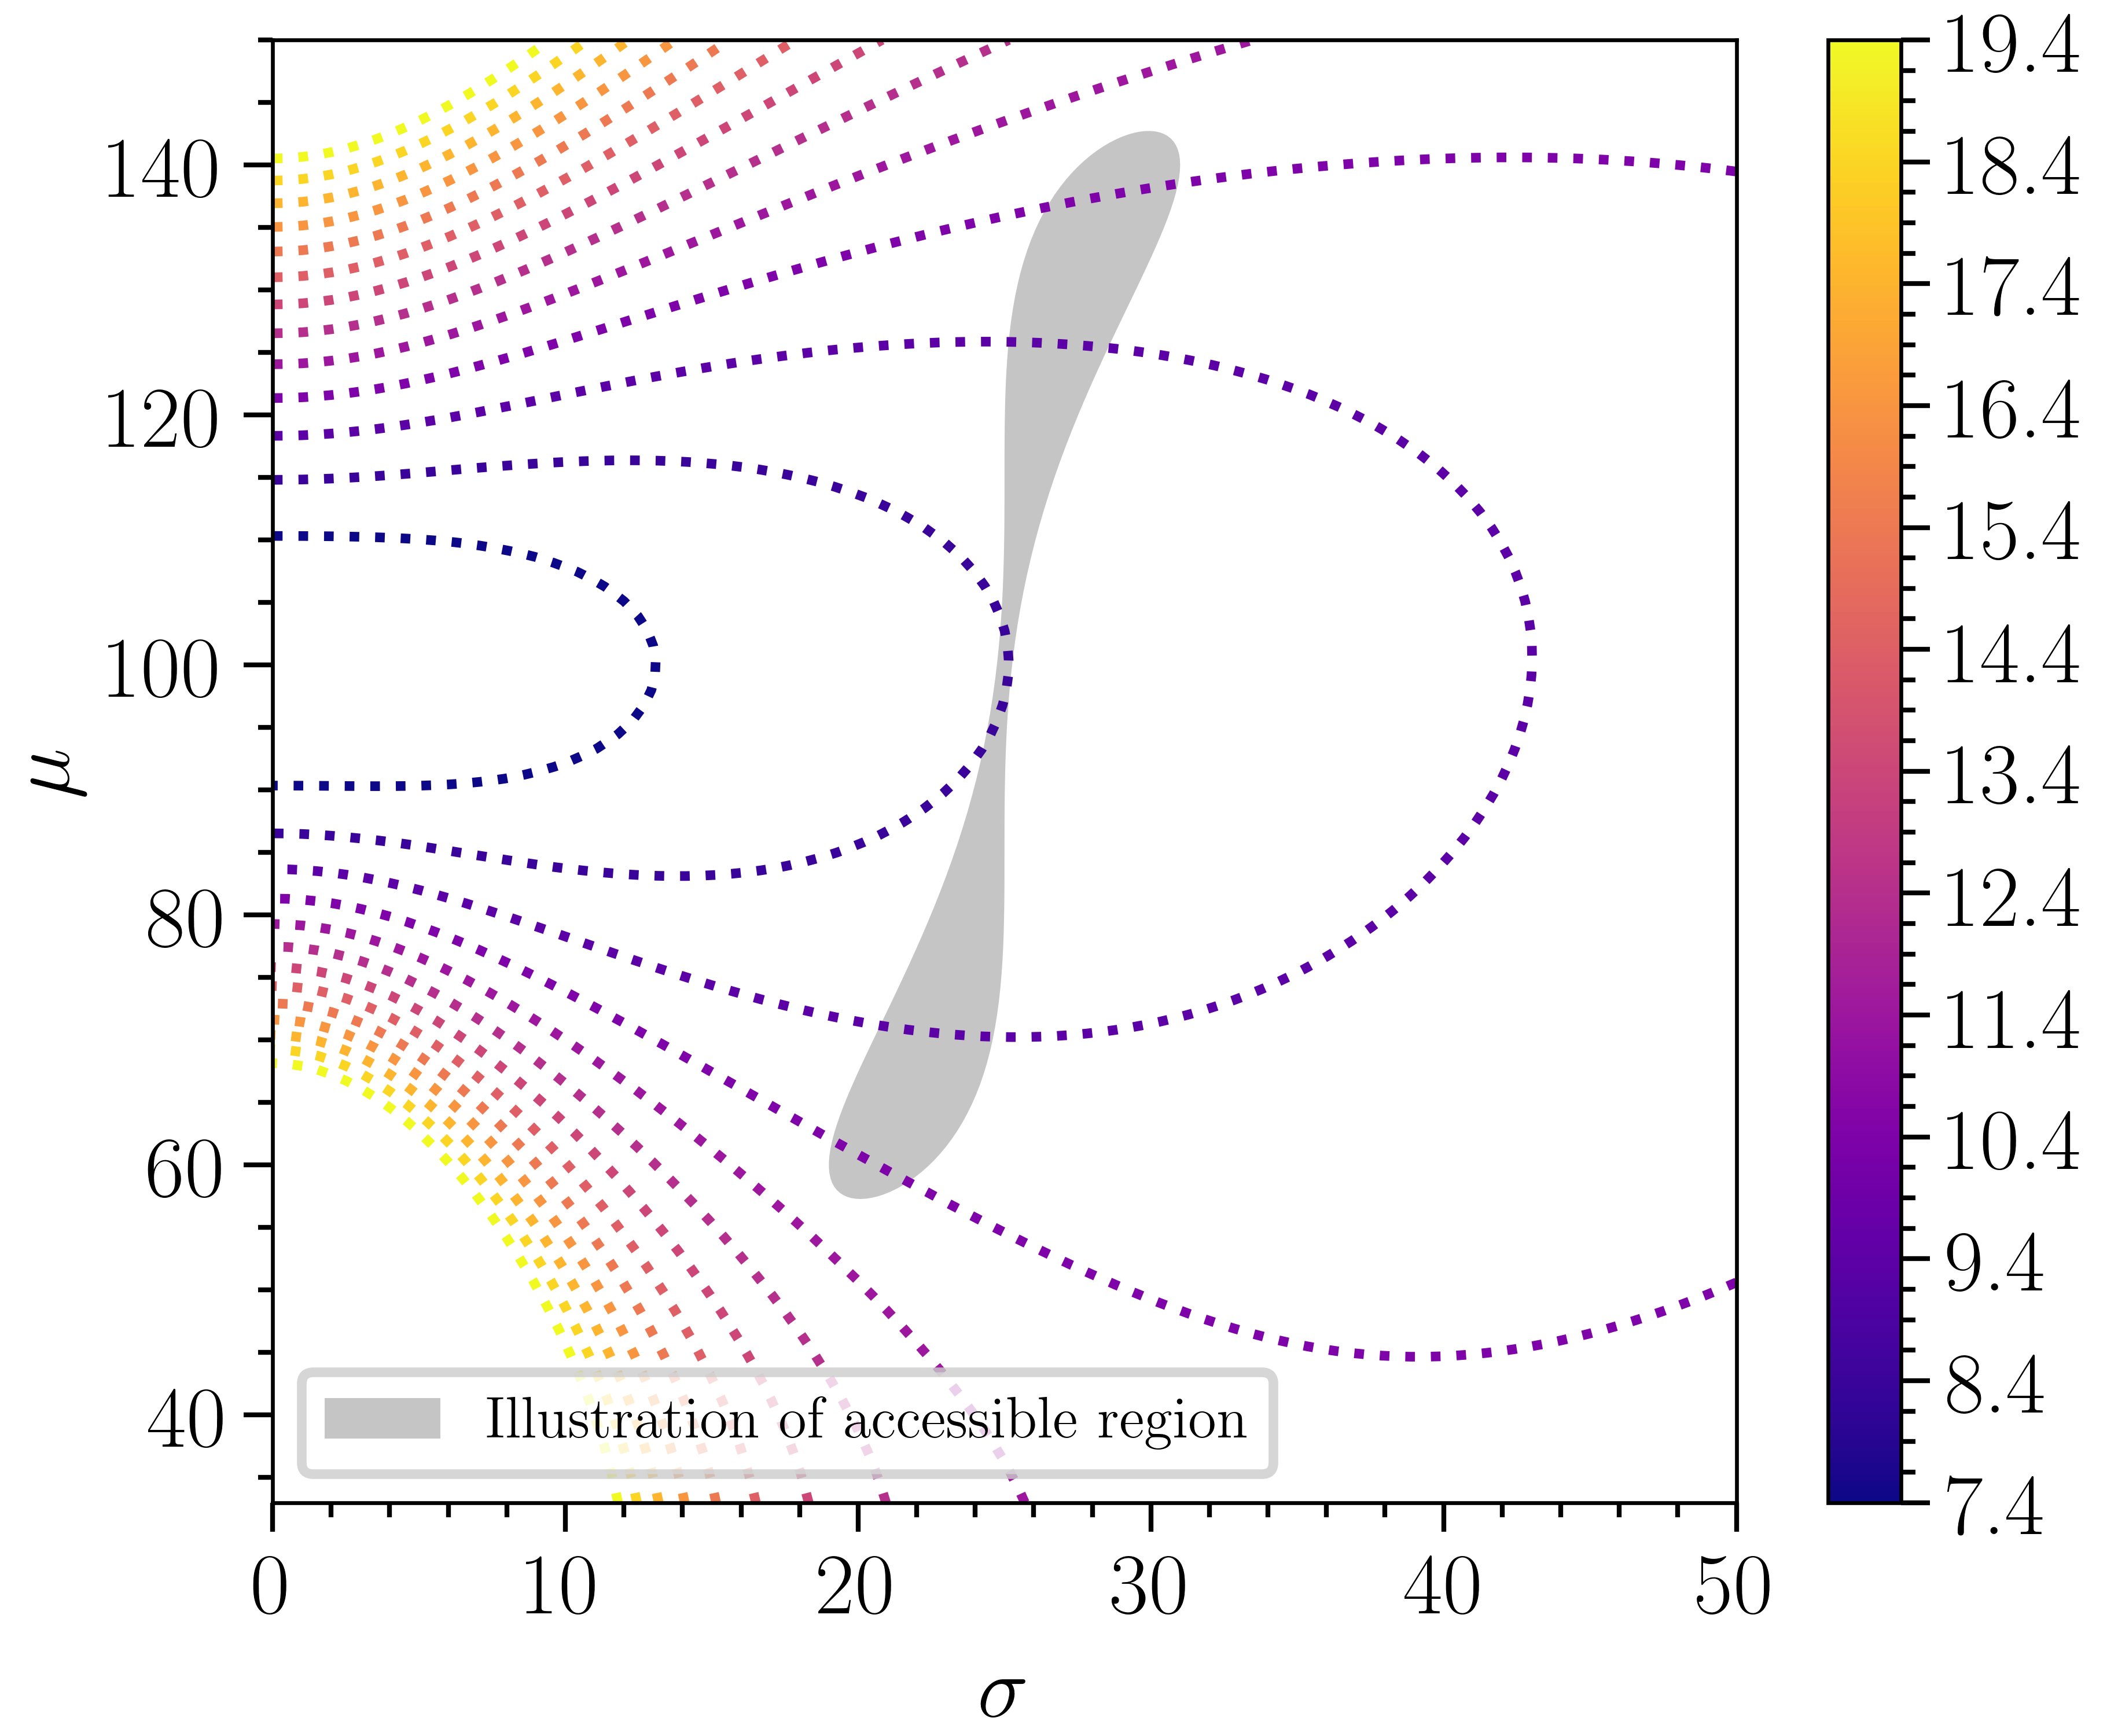
\includegraphics[width=0.5856\linewidth]{fig/fig1_contour}
\caption{\textbf{\textit{Likelihood contours and accessible region.}} Contours of constant $\lmc(\mu,\sigma|k=100)$.
The accessible region (gray) illustrates where values of $\mu$ and $\sigma$ may lie for a hypothetical physics model.
A minimization over $\vectheta$ can be thought of as a constrained minimization over the accessible region in $\mu$ and $\sigma$.
Note that as $\sigma$ increases the contours broaden.}
\label{fig:contour}
\end{figure}

It is instructive to examine the behavior of $\mcl$ for a single bin.
It is standard to work with the log-likelihood $l(\mu,\sigma|k) \equiv -2\ln \like(\mu, \sigma|k)$ and we do so here.
Figure \ref{fig:contour} shows the contour lines for $\lmc(\mu,\sigma|k=100)$.
Since $\mu$ and $\sigma$ are both dependent on the same underlying parameters, $\vectheta$, a minimization over $\vectheta$ can be thought of as a constrained minimization over $\mu$ and $\sigma$.
This is visualized as the gray region in Fig.~\ref{fig:contour}, which indicates where $\mu$ and $\sigma$ are allowed to vary for some physics model\footnote{A general bound for positive weights is $\sigma \leq \mu \leq \sigma \sqrt{m}$ which can be seen from their definitions.}.
Similarly, we can also visualize the standard Poisson log-likelihood, $\lpoisson(\mu|k=100)$, which is simply $\lmc$ constrained along the line $\sigma=0$.
%In the case of multiple bins, the likelihood is a superposition of the likelihood in each bin.

\begin{figure}[htp]
\centering
\centering
    \subfloat{
        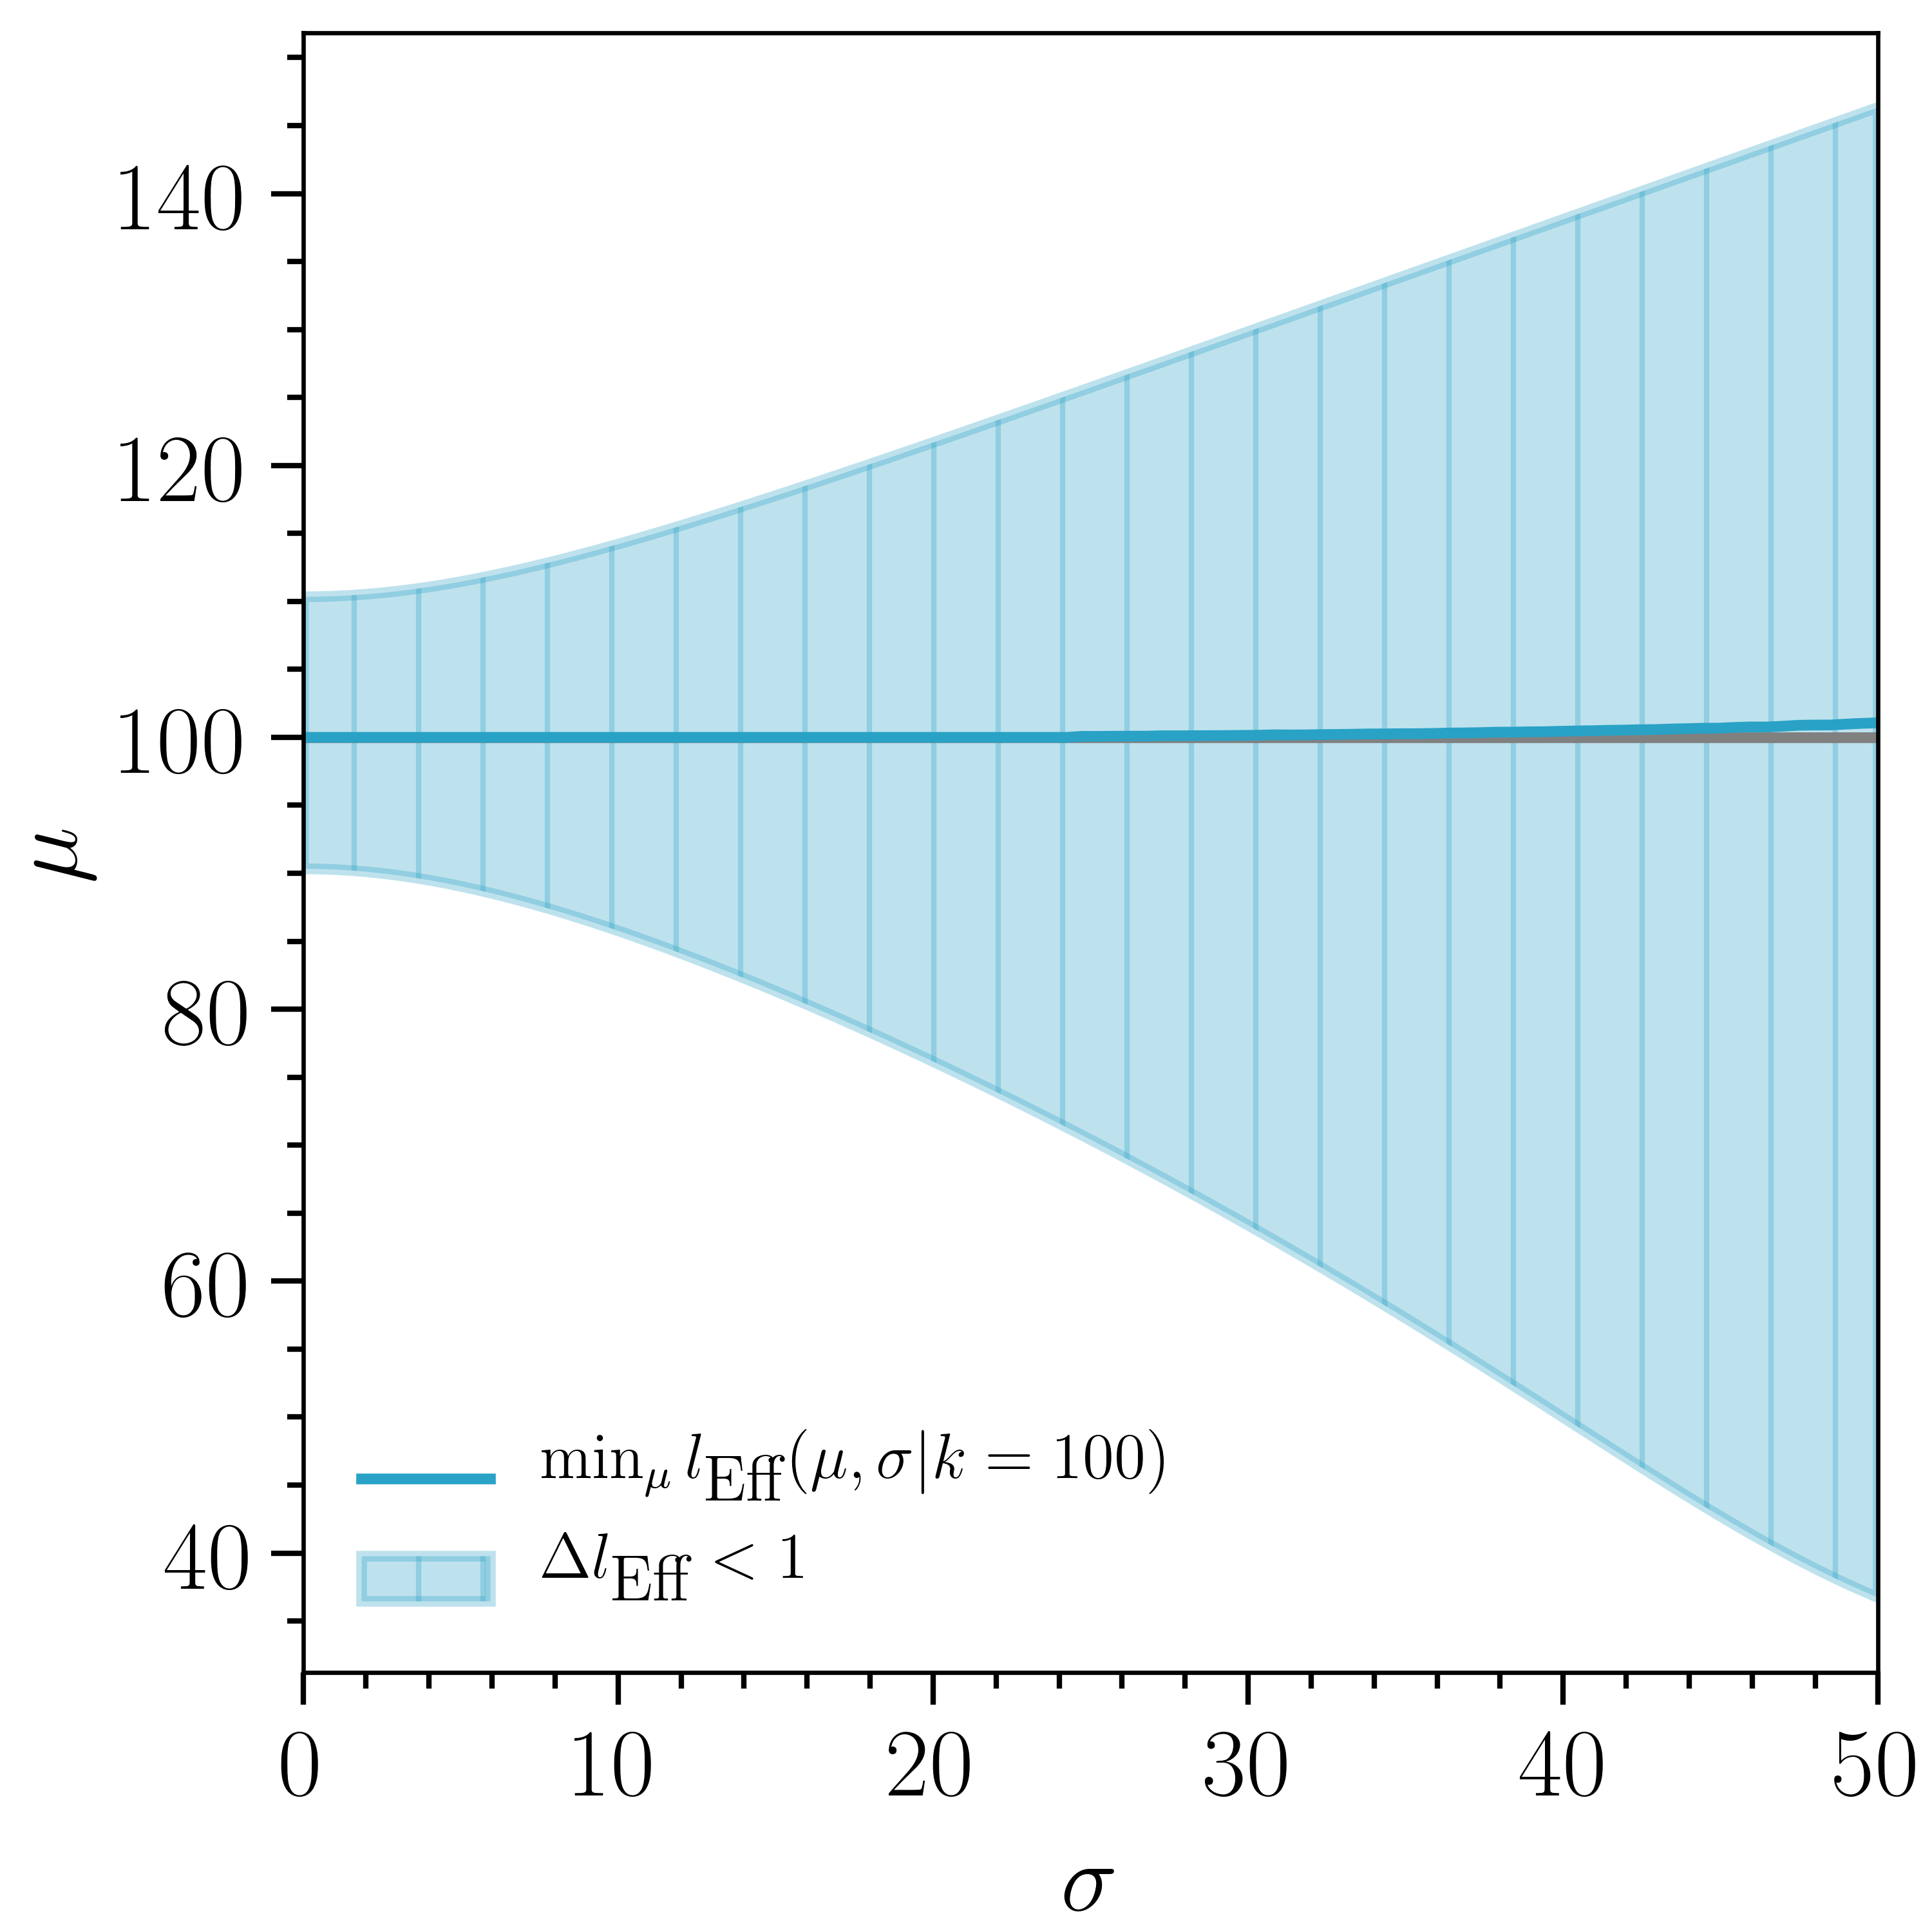
\includegraphics[width=0.48\linewidth]{fig/fig2_sigma}
    }
    \subfloat{
        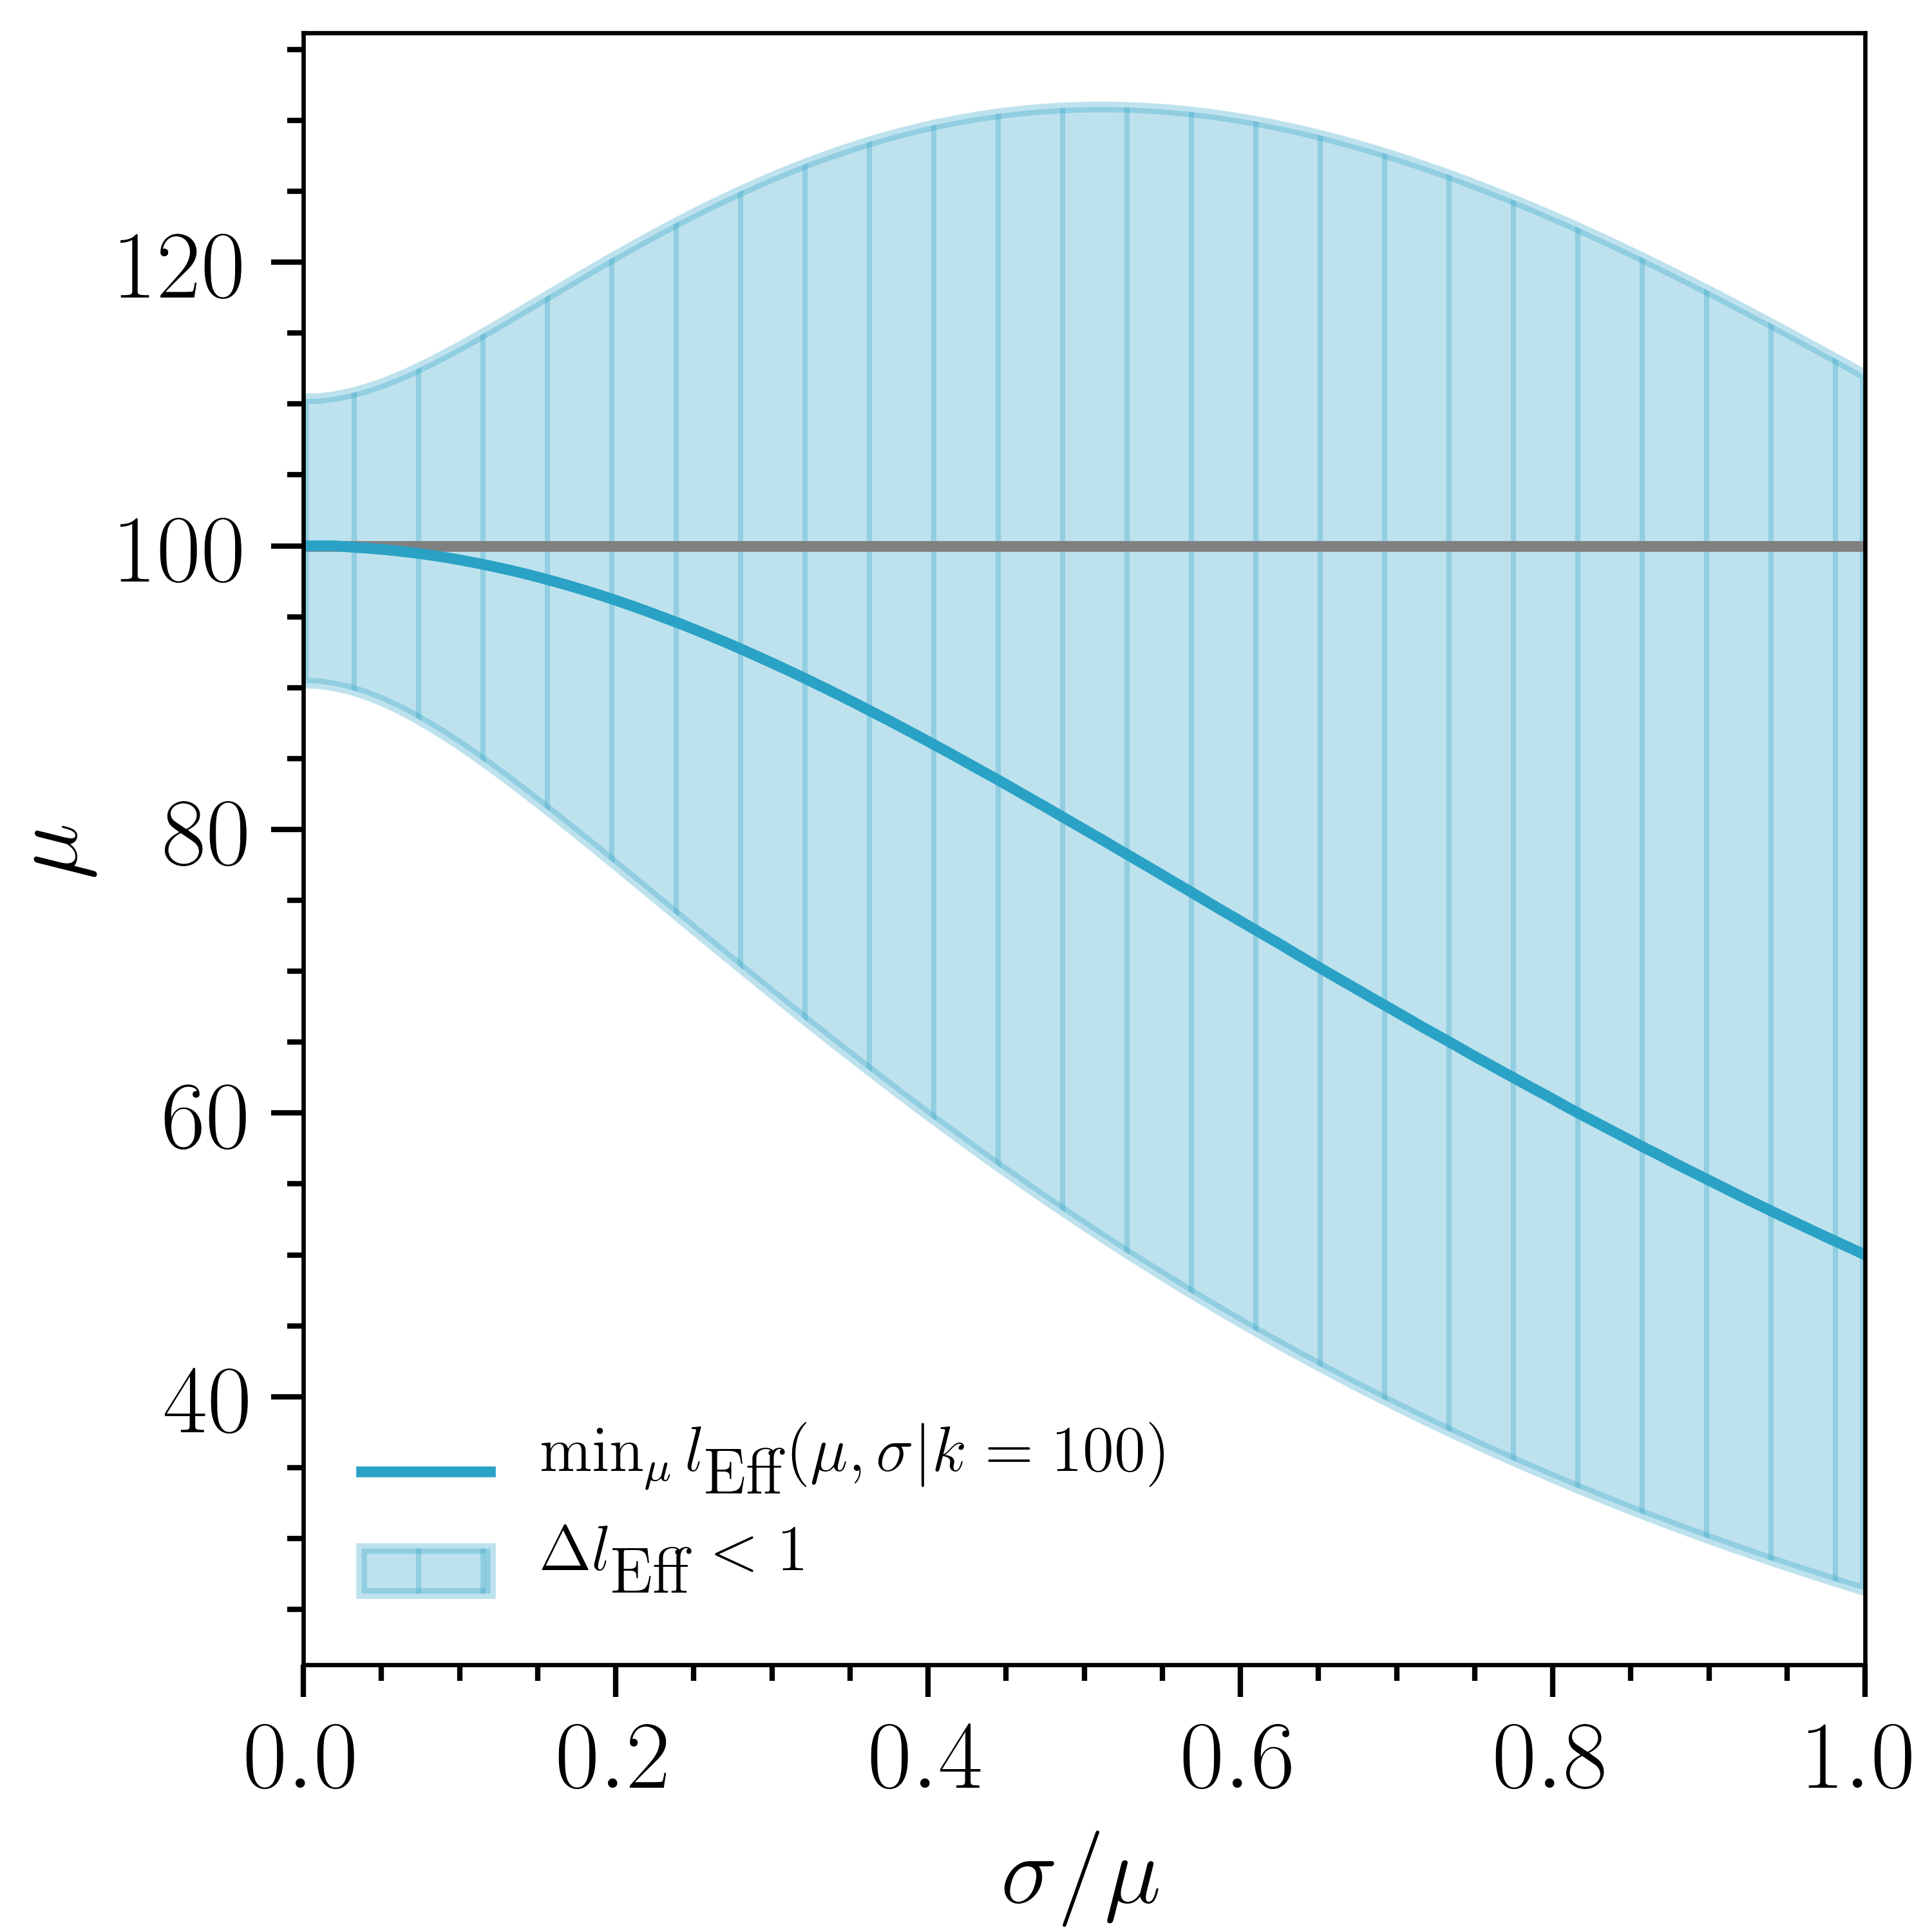
\includegraphics[width=0.48\linewidth]{fig/fig2_f}
    }
\caption{\textbf{\textit{Slices of $\lmc$ for two accessible regions.}} This figure shows $\lmc(\mu, \sigma|k=100)$ minimized over $\mu$ while $\sigma$ (left) and $\sigma/\mu$ (right) are held fixed.
The minimum, $\hatmc$, is shown as the solid blue line running through the center of the shaded regions.
The shaded regions indicate where $\lmc(\mu, \sigma|k) - \lmc(\hatmc, \sigma|k) < 1$.
As $\sigma$ goes to zero, the Poisson best-fit $\hatpoisson=100$ is obtained.
For fixed $\sigma/\mu$, $\hatmc$ deviates from $\hatpoisson$ as $\sigma/\mu$ increases.}
\label{fig:llhmin}
\end{figure}

To further illustrate the effect of the accessible region, we minimize $\lmc$ over $\mu$ for two possible constraints: fixed $\sigma$ and fixed $\sigma/\mu$.
In terms of Eq.~\eqref{eq:musigma}, a sufficient but not necessary condition for constant $\sigma/\mu$ with varying $\mu$ is equal weights, and a necessary but not sufficient condition for constant $\sigma$ with varying $\mu$ is $m \geq 2$.
For a standard Poisson likelihood, $\hatpoisson\equiv \min_\mu\lpoisson(\mu|k) = k$.
Figure \ref{fig:llhmin} shows $\hatmc \equiv \min_\mu \lmc(\mu,\sigma|k=100)$ as well as the region where $\lmc(\mu, \sigma|k) - \lmc(\hatmu, \sigma|k) < 1$ for fixed $\sigma$ (left) and fixed $\sigma/\mu$ (right).
Note that the shaded regions for fixed $\sigma$ are calculated without requiring that $\mu \geq \sigma$, which would be the case for Eq.~\eqref{eq:musigma}.
As $\sigma$ goes to zero, the Poisson best-fit and Wilks' $1\sigma$ interval are recovered.
As $\sigma$ or $\sigma/\mu$ increases, the shaded region becomes wider, as expected.
For fixed $\sigma$, $\hatmc$ does not deviate much from $\hatpoisson$, while for fixed $\sigma/\mu$, $\hatmc$ deviates from $\hatpoisson$ as $\sigma/\mu$ increases.
The shaded regions correspond to the $1\sigma$ interval assuming the approximation from Wilks' theorem and give a sense of the shape of $\mcl$ projected onto one-dimensional slices.
